\documentclass{beamer}
    \usefonttheme{serif}
\usepackage[backend=biber,sortcites,maxcitenames=1,maxbibnames=2]{biblatex}
    \addbibresource{./references.bib}
    \renewcommand*{\bibfont}{\tiny}

\usepackage{fontspec}
    \setmainfont{MLMRoman10}
    \setsansfont{MLMSans10}
    \setmonofont{MLMMono10}
\usepackage{verbatim}
\usepackage{tikz}
    \usetikzlibrary{positioning, arrows.meta}
\usepackage{xeCJK}

\title{Is Detokenization All In The Head?}
\author{Gustaf Gren}
\date{Methodology}

\begin{document}

\begin{frame}
  \titlepage
\end{frame}

\begin{frame}{Detokenization in LLMs}

Subword tokenization can split words into non-optimal fragments. But models seem to reconstruct whole words/concepts internally, called \textit{detokenization}\parencite{elhage2022a}.

\bigskip

Early layers \textbf{partially reverse the tokenization process} by combining subtokens into more coherent segments\parencite{lad2024,ferrando2024}.

\bigskip

\textcite{kaplan2025} propose the process is two-fold:
\begin{enumerate}
\item \textbf{Attention:} gathers the relevant pieces\parencite{ferrando2024, lad2024, elhage2022a}
\item \textbf{FFN:} maps them to the model's internal representation\parencite{geva2022}
\end{enumerate}

\end{frame}

\begin{frame}{Detokenization in LLMs}
\begin{itemize}
\item Are there crucial attention heads/circuits responsible?
\item Are the heads consistent across languages, and/or tokenizers?
\end{itemize}
\end{frame}

\begin{frame}{Data}

\begin{block}{Universal Dependencies PUD \parencite{nivre2020, akhundjanova2025}}
\begin{itemize}
\item Multilingual parallel manually annotated syntactic dataset. News/Wikipedia.
\item 1000 sequences, $\sim$ 20,000 words/language.
\item Used to control cross-language comparisons.
\end{itemize}
\end{block}

\end{frame}

\begin{frame}{Data Processing}

\textcite{kaplan2025} compared single-token to multi-token words. In multi-token words, attention flows more within the word compared to the single token control

\begin{center}
\begin{columns}
\column{0.4\textwidth}
\begin{block}{Multi-token words}
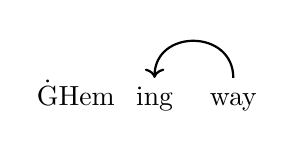
\begin{tikzpicture}[baseline, every node/.style={text height=1.5ex, text depth=.25ex}]
\node (1) {ĠHem};
\node (2) [right of=1] {ing};
\node (3) [right of=2] {way};
\draw[->, thick] (3.north) to[out=90,in=90,looseness=1.6] (2.north);
\end{tikzpicture}
\end{block}

\column{0.4\textwidth}
\begin{block}{Single-token words}
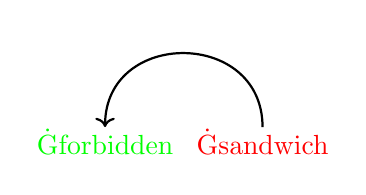
\begin{tikzpicture}[baseline, every node/.style={text height=1.5ex, text depth=.25ex}, node distance=2cm]
\node (1) {\textcolor{green}{Ġforbidden}};
\node (2) [right of=1] {\textcolor{red}{Ġsandwich}};
\draw[->, thick] (2.north) to[out=90,in=90,looseness=1.6] (1.north);
\end{tikzpicture}
\end{block}

\end{columns}
\end{center}

\end{frame}

\begin{frame}{Data Processing}

\begin{itemize}
\item \textbf{Problem:} token counts are not comparable across languages and tokenizers.
\item \textbf{Proposition:} compare attention within- vs across- UD word boundaries.
\end{itemize}

\bigskip
\begin{center}
\begin{columns}
\column{0.45\textwidth}
\begin{block}{In-boundary}
\textit{Last sub-token in a UD-word $\rightarrow$ penultimate subtoken} \\
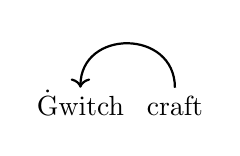
\begin{tikzpicture}[baseline, every node/.style={text height=1.5ex, text depth=.25ex}, node distance=1.2cm]
\node (1) {Ġwitch};
\node (2) [right of=1] {craft};
\draw[->, thick] (2.north) to[out=90,in=90,looseness=1.6] (1.north);
\end{tikzpicture}
\end{block}

\column{0.45\textwidth}
\begin{block}{Out-boundary}
\textit{First sub-token in a UD-word $\rightarrow$ last-subtoken in previous UD-word} \\
\begin{tikzpicture}[baseline, every node/.style={text height=1.5ex, text depth=.25ex}]
\node (1) {\textcolor{green}{於}};
\node (2) [right of=1] {\textcolor{red}{當}};
\node (3) [right of=2] {\textcolor{red}{時}};
\draw[->, thick] (2.north) to[out=90,in=90,looseness=1.6] (1.north);
\end{tikzpicture}
\end{block}

\end{columns}
\end{center}
\end{frame}

\begin{frame}{Raw Attention Preliminary Results}

Consistent with \textcite{kaplan2025}: \textbf{last subtokens attend strongly within word boundaries}.

\bigskip
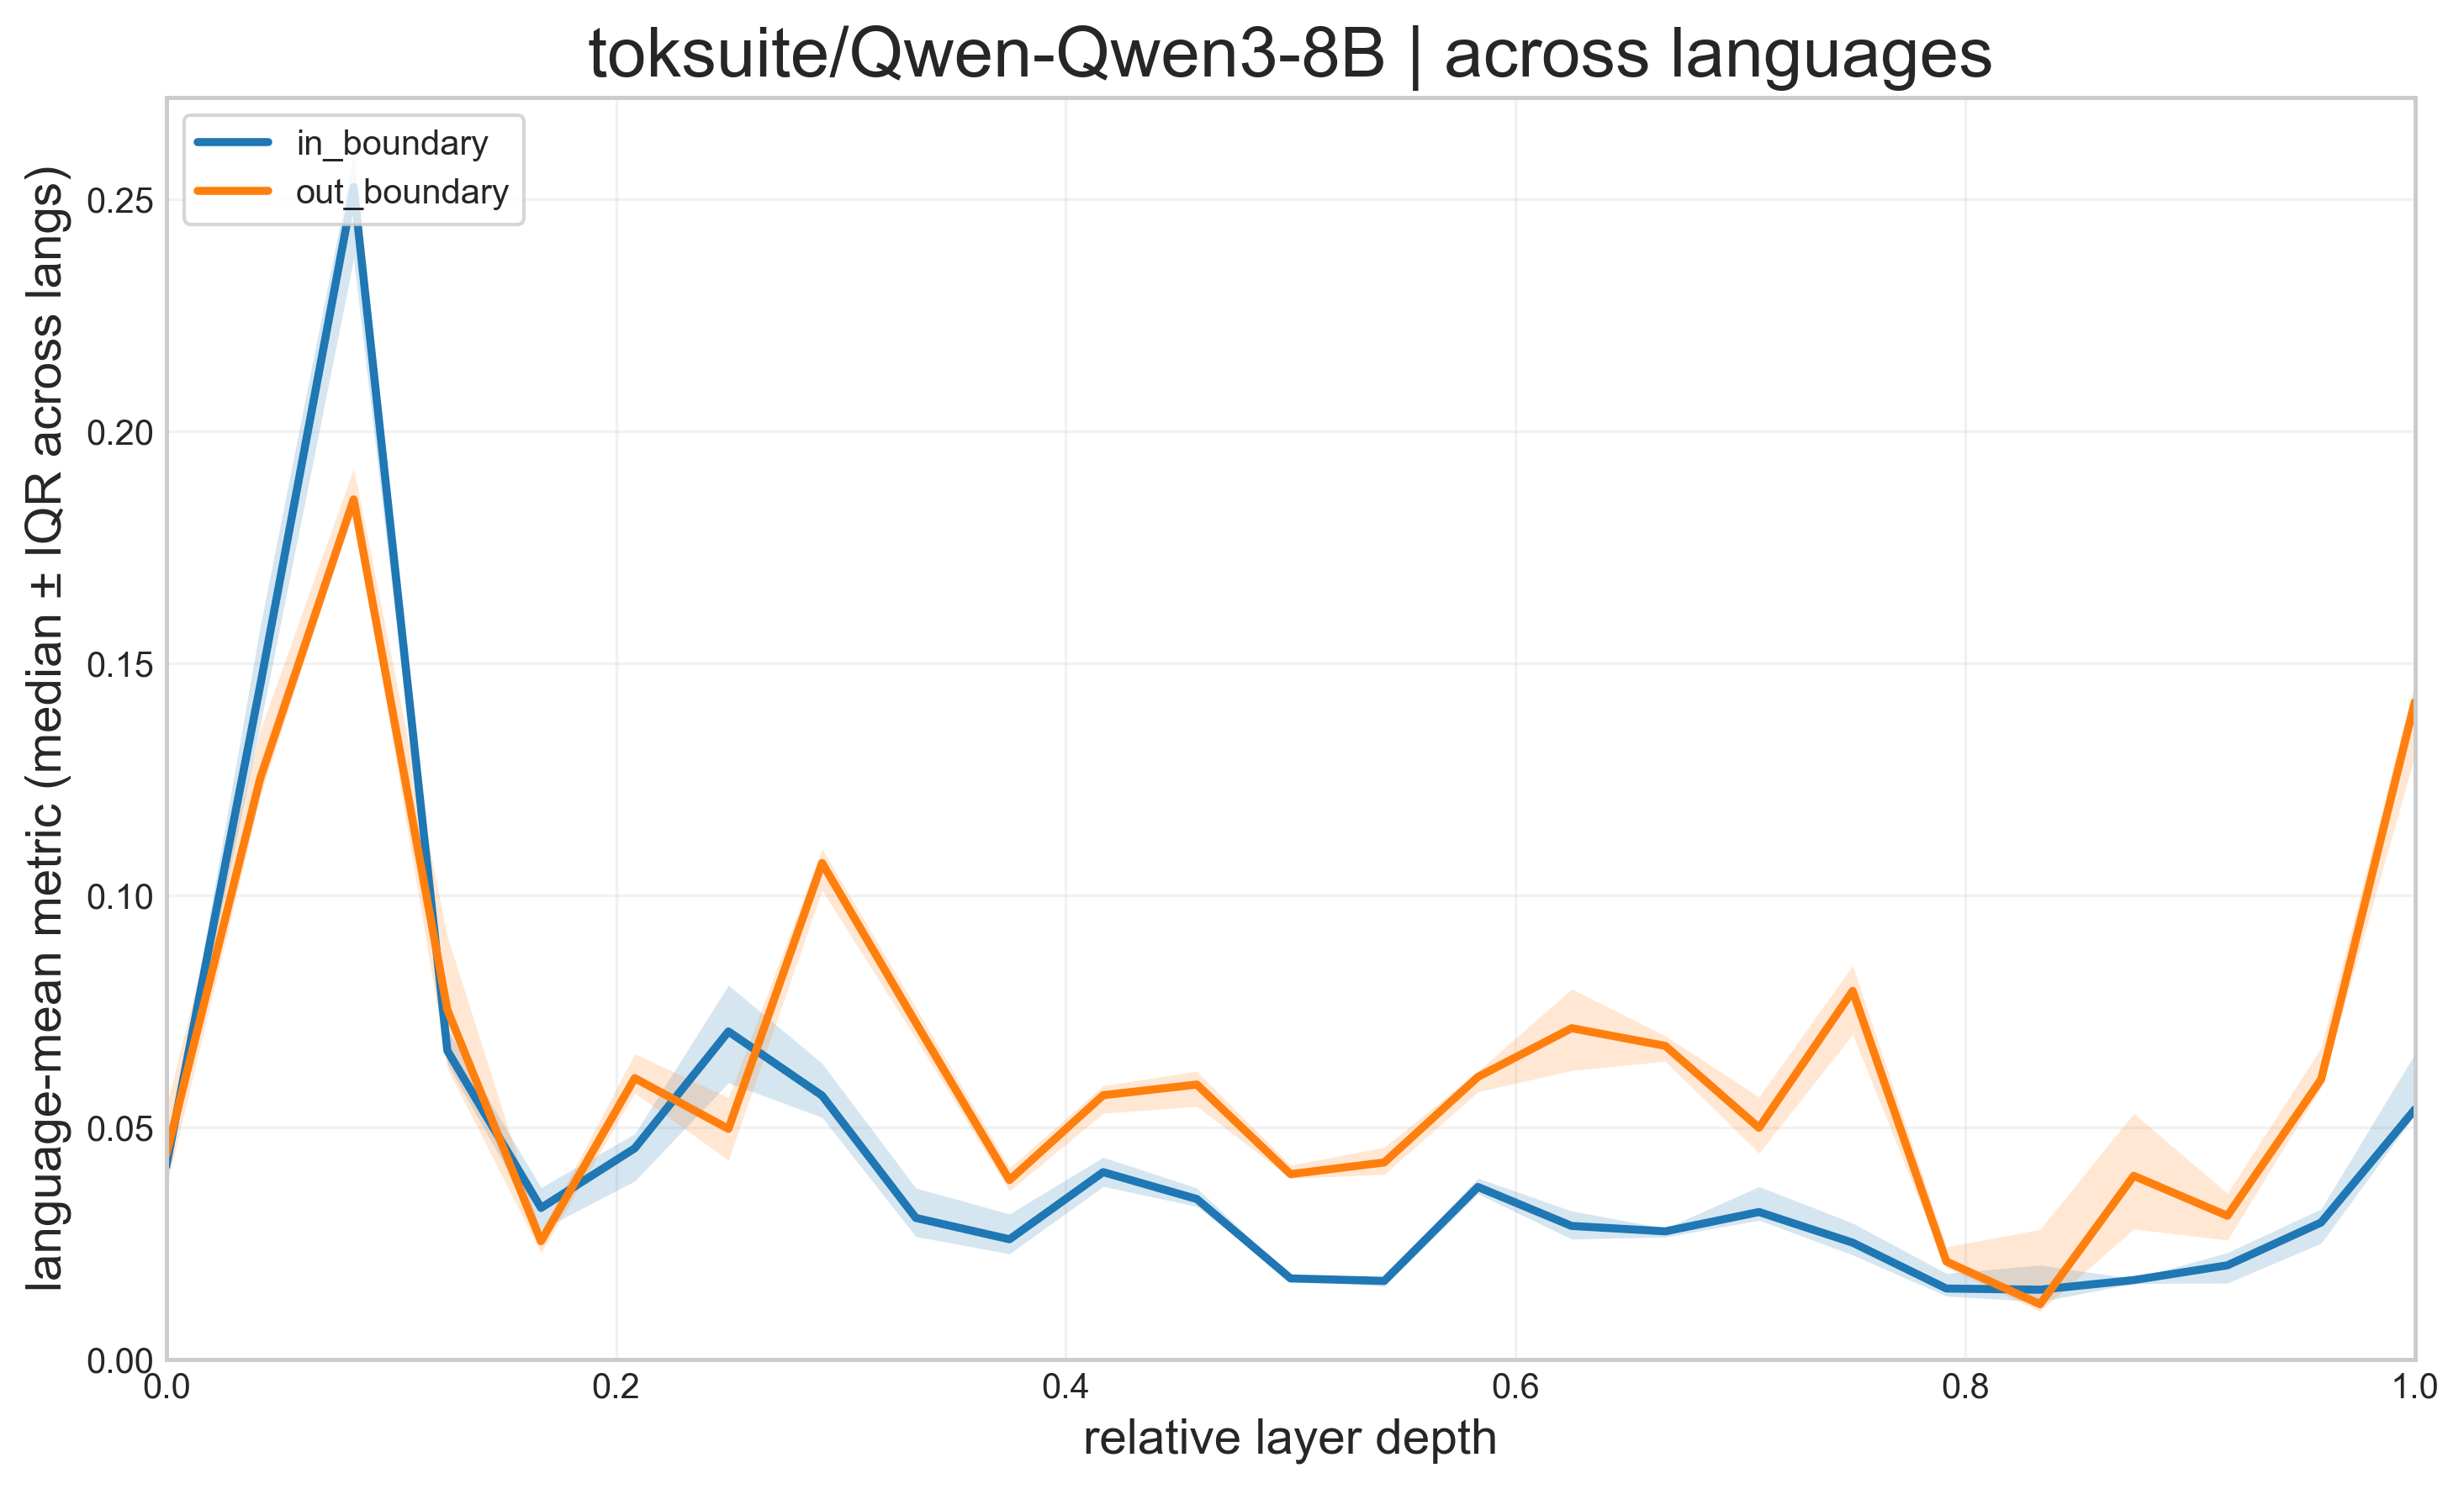
\includegraphics[width=\textwidth]{fig/mode_comparison_across_languages.png}
\end{frame}

\begin{frame}{Attention Head Patterns Preliminary Results}
\textbf{Certain attention heads seem to prefer in-word attention}:\\
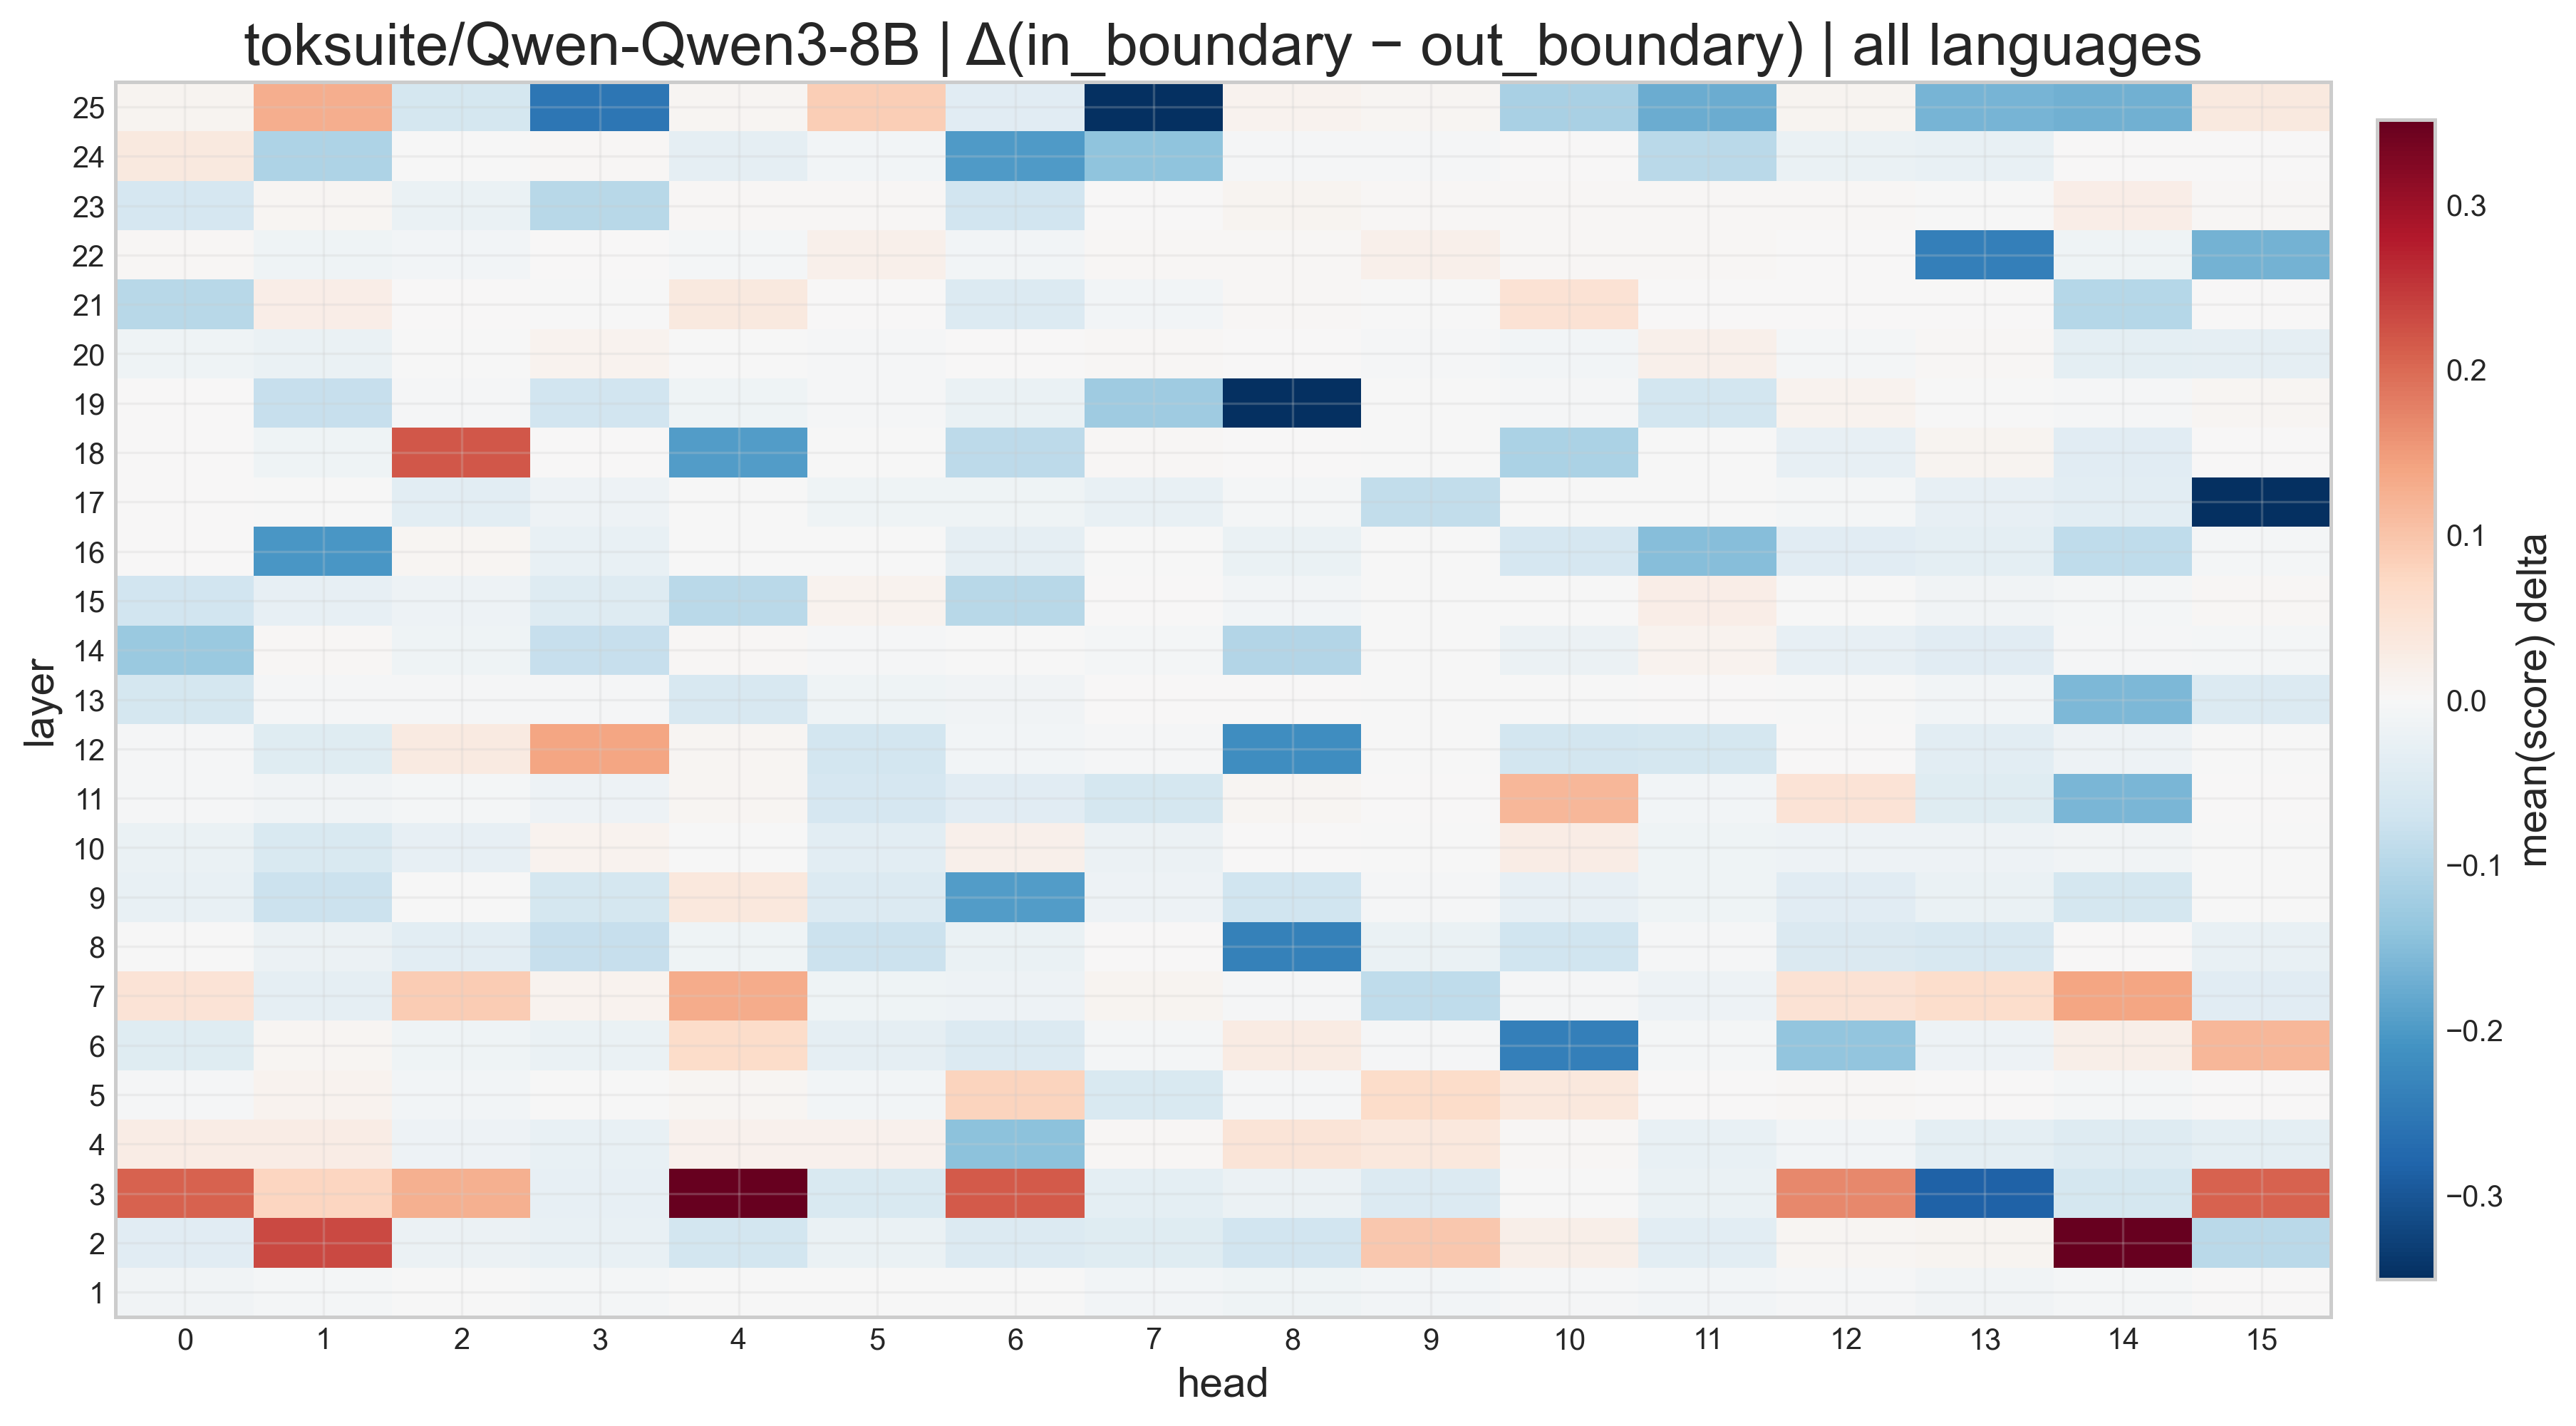
\includegraphics[width=\textwidth]{fig/heatmap_delta_in_boundary_minus_out_boundary_alllangs.png}
\end{frame}

\begin{frame}{What's Next?}

\begin{itemize}
    \item Are identified heads \textbf{necessary for detokenization}?
    \item Compare:
    \begin{itemize}
        \item clean model
        \item targeted head ablation
        \item random head ablation
    \end{itemize}
    \item Evaluate using \textbf{activation patching} (\textbf{word retrieval}) across layers/components.
\end{itemize}
\end{frame}

\begin{frame}{Hypothesis}

If \textit{detokenization} occurs, \textbf{retrieval should primarily be located in the early layers}.

\begin{description}
    \item[\textbf{H}] Effect will be disproportionally affected by ablating targeted attention heads rather than random and clean control.
    \item[\textbf{H}] Effect will be pronounced in the FFN component, as found by \textcite{kaplan2025}.
\end{description}
\end{frame}

\begin{frame}[allowframebreaks]{References}
\printbibliography
\end{frame}

\begin{frame}{Preliminary Significance Testing - TokSuite}
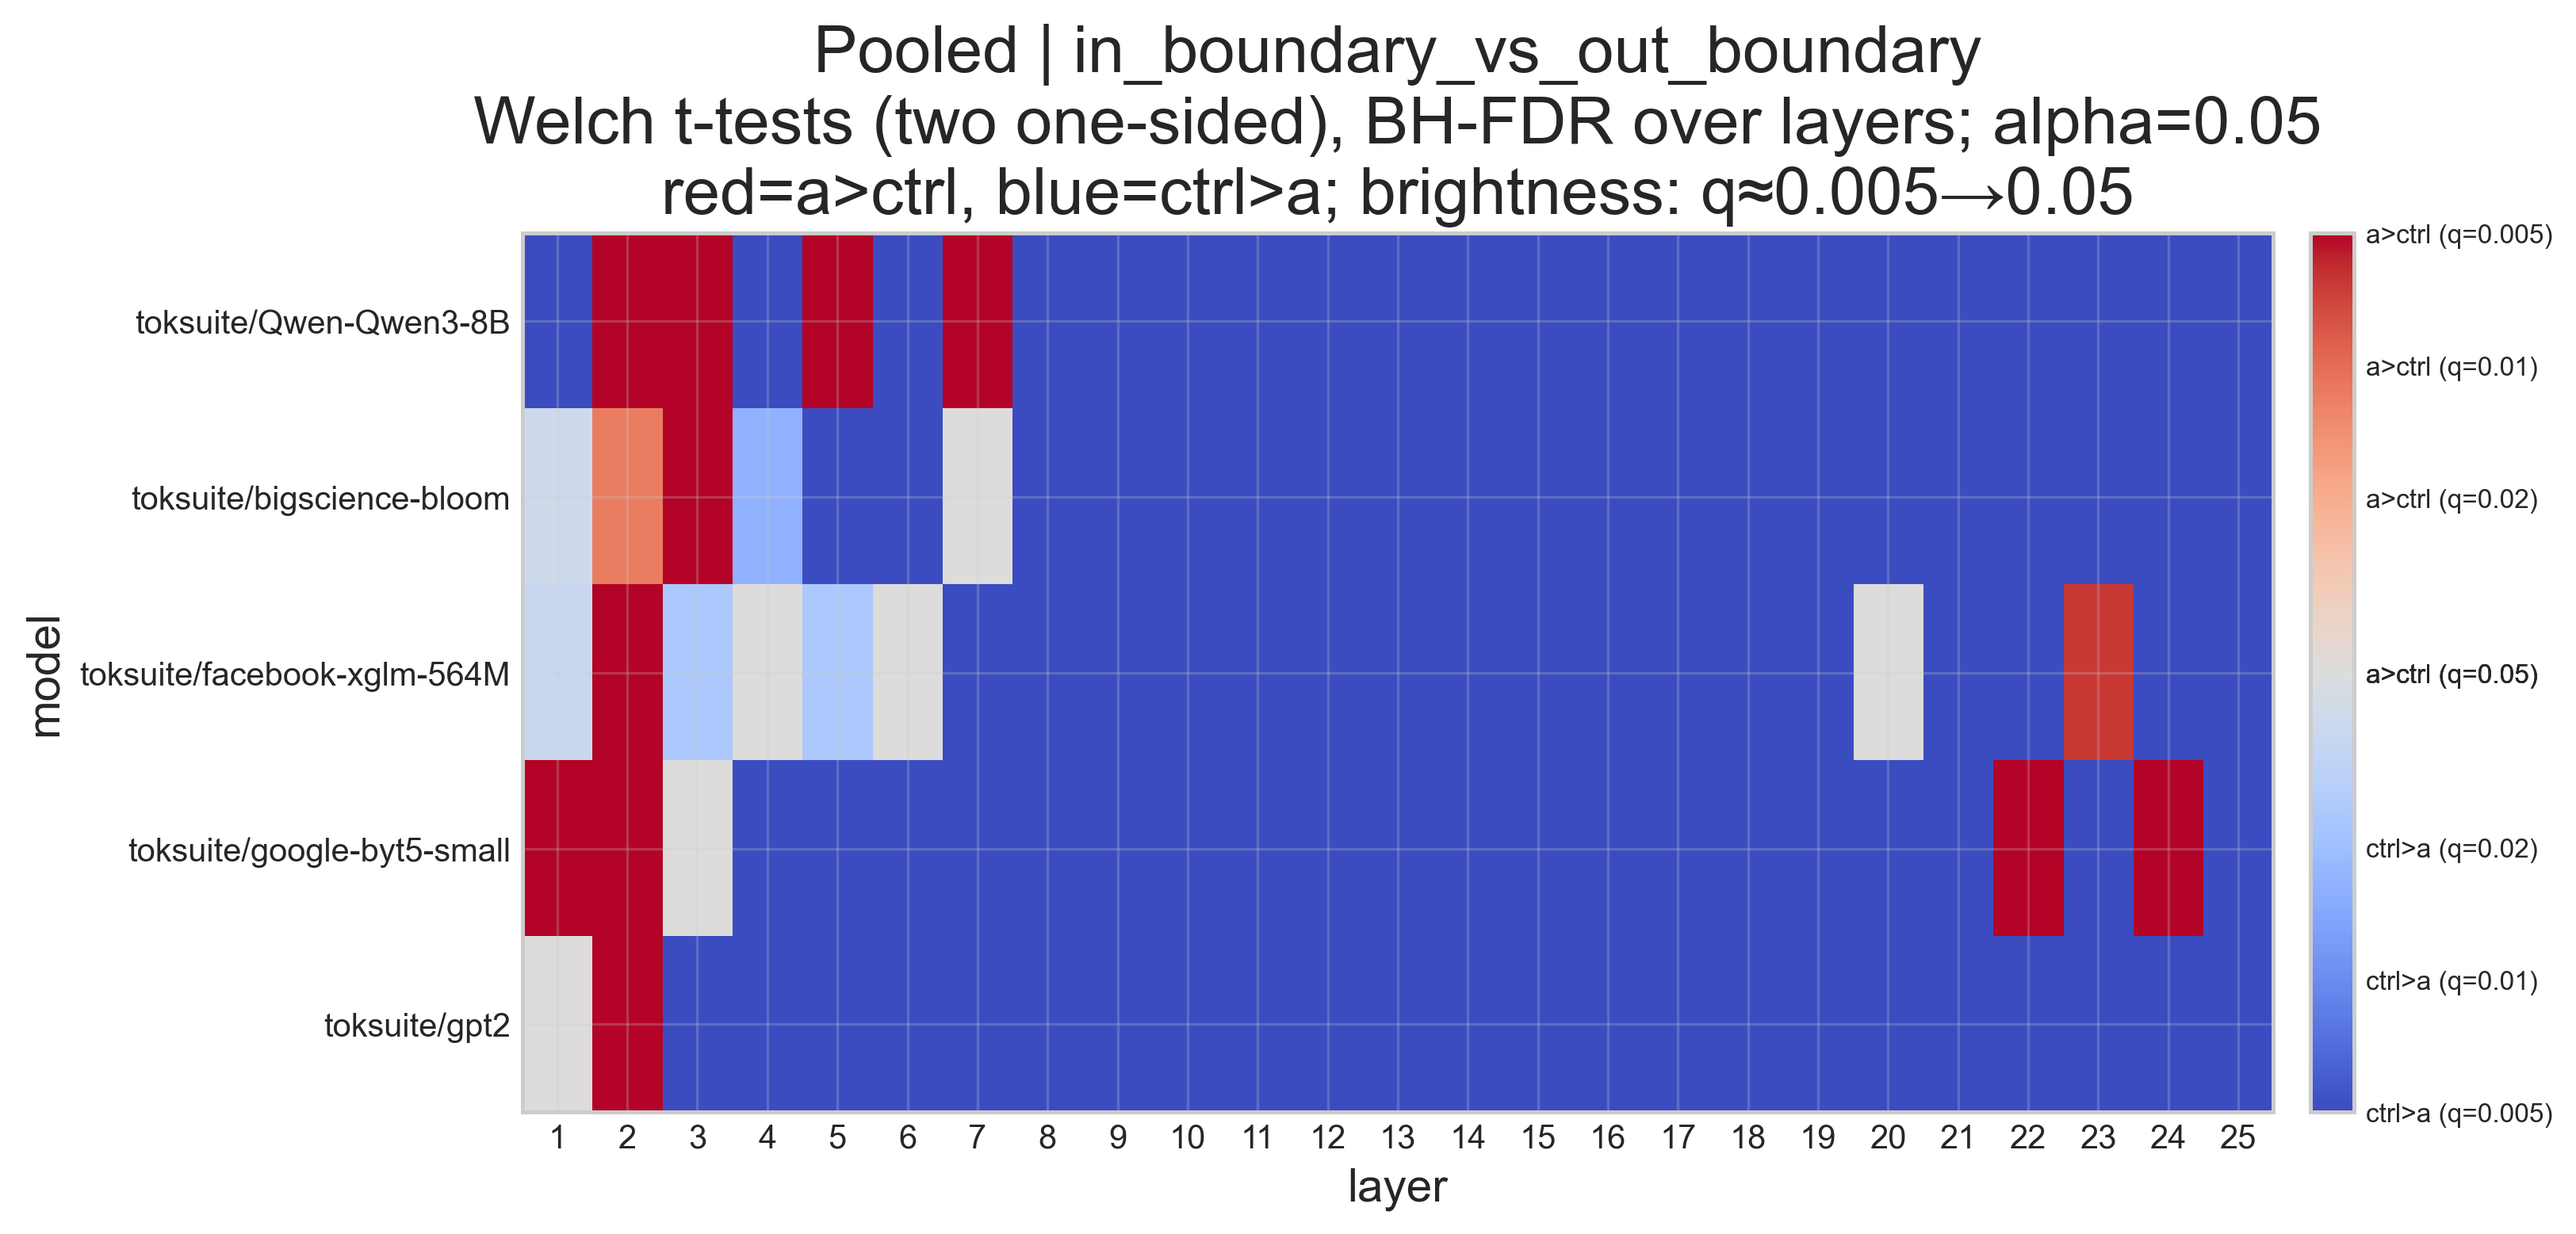
\includegraphics[width=\textwidth]{fig/heatmap_in_boundary_vs_out_boundary.png}
\end{frame}

\begin{frame}{Activation Patching}

\textbf{Goal:} Identify which model components causally influence a behavior.

\begin{itemize}
    \item Run a \textbf{clean forward pass} and save internal activations.
    \item Replace activations in another run with the saved ones.
    \item Measure how the output changes.
\end{itemize}

\begin{block}{\textbf{PatchScopes} \parencite{ghandeharioun2024}}
\begin{itemize}
    \item Activation patching via \textbf{prompting}.
    \item Example prompt: \\
    \textit{``Repeat this word twice: 1) X 2)''}
    \item Replace the token embedding for $X$ with a representation from a specific component and layer.
    \item Observe how the model completes the prompt.
\end{itemize}

\end{block}

\end{frame}

\begin{frame}{Transformer block}
\begin{tabular}{lcl}
& $h_{l-1}$ & \\
& | & \\
& Multi-head Attention & \\
& | & \\
& Residual + Norm & \\
& | & \\
& FFN & \\
& | & \\
& Residual + Norm & \\
& | & \\
& $h_l$ & (hidden representation for layer $l$)
\end{tabular}
\end{frame}

\end{document}
